\documentclass{report}   	% use "amsart" instead of "article" for AMSLaTeX format
\usepackage{geometry}                		% See geometry.pdf to learn the layout options. There are lots.
\geometry{a4paper, margin=1in}                   		% ... or a4paper or a5paper or ... 
%\geometry{landscape}                		% Activate for rotated page geometry
%\usepackage[parfill]{parskip}    		% Activate to begin paragraphs with an empty line rather than an indent
\usepackage{graphicx}				% Use pdf, png, jpg, or eps§ with pdflatex; use eps in DVI mode
								% TeX will automatically convert eps --> pdf in pdflatex		
\usepackage{amssymb}
\usepackage{enumitem}
\usepackage{graphicx}
\usepackage{pdflscape}
\usepackage{longtable}

\renewcommand{\chaptername}{Section}

%SetFonts

%SetFonts


\title{Phase 1}
\author{Team Fractal}
\date{}							% Activate to display a given date or no date

\begin{document}
\maketitle

\chapter{Requirements}
\section{Background}

% \section{User Stories} (in requirements-table.tex)
\newgeometry{left=0.75in, right=0.75in, top=1in, bottom=1in}
\begin{landscape}
	\section{User Stories}
	\begin{longtable}{|l||l|p{4cm}|p{8cm}|p{7cm}|}
		\hline
		\# & Title & Story & Functional & Non-functional \\ \hline \hline \endhead
		1 & GUI & As a player I must be able to see a GUI consisting of a map subdivided into plots and should be able to gain information about the state of my freehold and my individual plots.
		& \begin{enumerate}[label=1.1.\arabic*.]
			\item The entire map should be available to the user
			\item Information about individual plots should be shown:
			\begin{enumerate}
				\item Which player owns a plot
				\item Output of ore, energy, and food
				\item Robiticons installed
			\end{enumerate}
		\end{enumerate}
		& \begin{enumerate}[label=1.2.\arabic*.]
			\item The map must represent the university of York with at least 3 identifiable landmarks
			\item The map must be split into multiple evenly sized plots
			\item Each player must be uniquely identifiable on the map
			\item The player must be able to access the whole map
			\item The GUI should load in less than 5 seconds
		\end{enumerate} \\ \hline
	
	2 & Purchasing Land
	& As a player I must be able to purchase plots of land to increase the size and productivity of my freehold
	& \begin{enumerate}[label=2.1.\arabic*.]
		\item The player must be able to exchange currency for more land during the acquisition phase of the round
	\end{enumerate}
	& \begin{enumerate}[label=2.2.\arabic*.]
		\item Plots will have different strengths and weaknesses in terms of production based on location and terrain type
		\item The player must be able to cancel a purchase to avoid accidental purchases
	\end{enumerate} \\ \hline

	3 & Plot Modification
	& As a player, I must be able to buy and sell various modifications to my plots to increase productivity and/or style.
	& \begin{enumerate}[label=3.1.\arabic*.]
		\item The system must provide a number of possible modifications to plots
	\end{enumerate}
	& \begin{enumerate}[label=3.2.\arabic*.]
		\item The player must be able to view all modifications and choose one to install
		\item Installation must take less than a second
	\end{enumerate} \\ \hline

	4 & Multiplayer
	& As a player, I must be able to buy and sell various modifications to my plots to increase productivity and/or style.
	& \begin{enumerate}[label=4.1.\arabic*.]
		\item A player must be able to chose whether to play against another human or the computer
		\item At least two users must be able to play the game together
		\item The players will take turns in playing
	\end{enumerate}
	& \begin{enumerate}[label=4.2.\arabic*.]
		\item The simulated player should take no longer than 20 seconds to complete a round
	\end{enumerate} \\ \hline

	5 & Round Structure
	& As a player I must be able to play the game in a structured manner
	& \begin{enumerate}[label=5.1.\arabic*.]
		\item The game must be split into multiple rounds
		\item Each round should be made of 5 phases:
		\begin{enumerate}[label=\arabic*.]
			\item Purchase any unoccupied plots
			\item Purchase and customise roboticons
			\item Install roboticons on plots of land
			\item The colony produces resources
			\item The player can buy and sell resources
		\end{enumerate}
		\item Phases 2 \& 3 must be time limited. 
	\end{enumerate}
	& \begin{enumerate}[label=5.2.\arabic*.]
		\item It must be easy for the player to move between phases
		\item Changes between phases must take no longer than 5 seconds
	\end{enumerate} \\ \hline

	6 & Roboticons
	& As a player I must be able to purchase and customise my roboticons so they can produce more of certain amounts of resources
	& \begin{enumerate}[label=6.1.\arabic*.]
		\item The player must be able to purchase roboticons from the market
		\item The market must have ore to produce roboticons
		\item The user must be able to purchase modifications for the robiticon at the market
		\item The user must be able to install modifications on roboticons 
		\item The user must have the option to install a roboticon on a plot of land they own.
	\end{enumerate}
	& \begin{enumerate}[label=6.2.\arabic*.]
		\item At the start of the game, the market has 12 roboticons
		\item The user should be able to tell how a roboticon they are installing will affect the plot it is installed on
	\end{enumerate} \\ \hline

	7 & Resources
	& As a player I must be able to produce resources from my plots
	& \begin{enumerate}[label=7.1.\arabic*.]
		\item Roboticons are required to produce resources
		\item During phase 4 the user’s roboticons will generate resources across the freehold
		\item Food, energy and ore will be generated
		\item Different amount of resources will affect the rate of production
	\end{enumerate}
	& \begin{enumerate}[label=7.2.\arabic*.]
		\item The resource production should not take more than 5 seconds
		\item The resource production should happen automatically
	\end{enumerate} \\ \hline

	8 & Buying/selling resources
	& As a player, I must be able to buy and sell resources to other players through an auction, or to the market at a fixed price so that I can maximise my wealth and productivity.
	& \begin{enumerate}[label=8.1.\arabic*.]
		\item The system must provide an auction facility, where the other player and the market bid for resources
		\item The system must choose a market price based on resource abundance
		\item The player must be able to buy/sell resources from/to other players, or the market
	\end{enumerate}
	& \begin{enumerate}[label=8.2.\arabic*.]
		\item At the start of the game, the market must have 16 units of food and energy and 0 units of ore
		\item At the start of the game, the player must have a small amount of money
	\end{enumerate} \\ \hline

	9 & Gambling
	& As a player, I must be able to enter the bar and either win or lose money.
	& \begin{enumerate}[label=9.1.\arabic*.]
		\item The system must provide a minigame where the player can gamble with their money
	\end{enumerate}
	& \begin{enumerate}[label=9.2.\arabic*.]
		\item The minigame must give feedback on the money won or lost
	\end{enumerate} \\ \hline

	10 & Winning
	& As a player, I must be able to win or lose the game.
	& \begin{enumerate}[label=10.1.\arabic*.]
		\item The system must assign a value to each resource at the end of the game, from which a player's final wealth is calculated
		\item The game must end on the round in which the last plot of land has been allocated.
		\item The player with the highest final wealth must be declared the winner, and Vice-Chancellor of the colony
	\end{enumerate} & \\ \hline
	\end{longtable}
The main risks associated with these requirements are risks 3, 4, 5 \& 6 as certain requirements may not be able to be implemented due to available tools or staff ability, however risks 8 and 11 must also be considered as they may change the requirements themselves.
\end{landscape}
\restoregeometry

\chapter{Architecture}
\section{Proposed Architecture}
\section{Justification}

\chapter{Method Selection and Planning}
\section{Proposed Software Engineering Methods}
\section{Team Organisation}
\section{Project Plan}

\chapter{Risk Assessment and Mitigation}
\section{Introduction}
Throughout the project we will face a number of potential risks however we will do our best to mitigate them.
When analysing the risks we will focus on two factors, likelihood and severity.

A risk can either have a high, medium, or low chance of becoming a reality.
If a problem is not likely to occur when running a project three times or more we deem it to have a low likelihood.
If it is likely to occur once during the project or when running a project twice we deem it medium likelihood.
Finally, if it is likely to occur multiple times during the project, we will deem it as high likelihood.

A risk can also either be high, medium, or low in severity.
A high severity risk could result in months of lost progress up to having to totally start over.
A medium severity risk could result in the loss of between one week and a few weeks of progress.
Finally a low severity risk would only result in a maximum of a few days of lost progress.

To combine these two factors into something meaningful we will use a risk matrix (Figure~\ref{fig:risktable}).
This will allow us to find a balance and identify the risks that will pose major problems.

\begin{figure}[h]
	\begin{centering}
		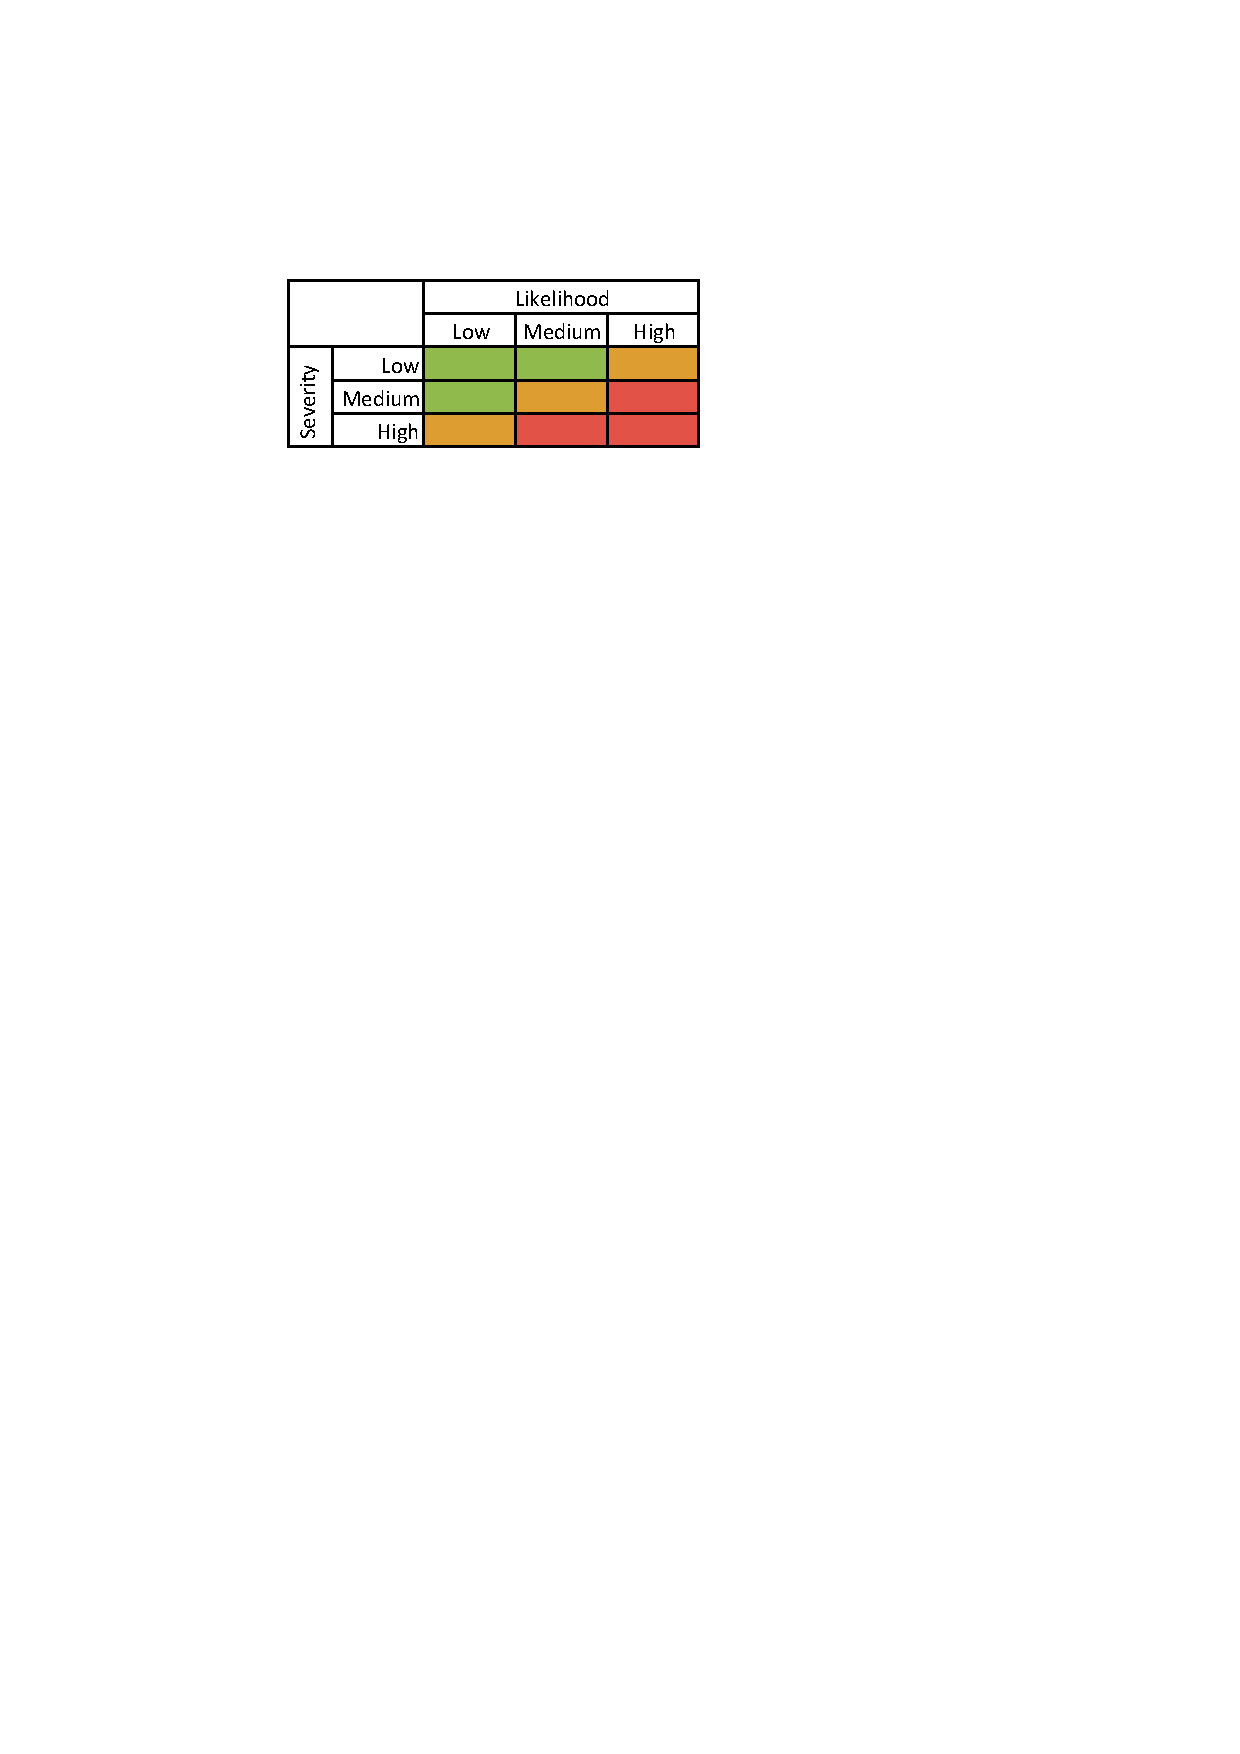
\includegraphics{risktable.pdf}
		\caption{Table showing how likelihood and severity of a risk combine to show overall impact of the risk}
		\label{fig:risktable}
	\end{centering}
\end{figure}

Green cells in the matrix are considered to be overall low risk, this is because they are not particularly likely to happen and if they do they will not have be severe enough to majorly impact the project.
Orange cells signify an overall medium risk.
They are either likely to happen but low severity, very unlikely to happen but would have a very severe impact or somewhere between.
Overall high severity risks, red cells, are the most important to mitigate.
They have a reasonably high chance of happening and could result in the loss of weeks or months of work.

It is important to categorise risks once they have been identified so that we can prioritise mitigation, it is imperative that overall high risks cannot happen and in the case that they do we must be able to cope with them and have protocols in place to lessen the impact.

We will be presenting the risks in a risk register with columns identifying, analysing and showing the mitigations for the risk.
This will give us an accessible and easily modifiable document which we will be able to use throughout the project when considering or attempting to mitigate risks.

\newpage
\section{Risk Assessment}

\end{document}  